\documentclass[output=paper]{langscibook}
\ChapterDOI{10.5281/zenodo.4545041}

\author{Aline Ferreira\affiliation{University of California, Santa Barbara} and Stefan Th. Gries\affiliation{University of California, Santa Barbara; Justus Liebig University Giessen} and  John W. Schwieter\affiliation{Wilfrid Laurier University}}

\title[Assessing indicators of cognitive effort in professional translators]{Assessing indicators of cognitive effort in professional translators: A study on language dominance and directionality}  

\abstract{Recently in translation studies, important advances have been made with respect to directionality (i.e., whether translation is done into one’s native or non-native language). What was once considered the “elephant in the room,” directionality now has a growing number of empirical studies that analyze factors which contribute differentially to translation. In this chapter, we review variables that have been previously identified as related to a higher or a lower degree of cognitive activity in direct and inverse translation (DT and IT, respectively). Against this backdrop, we present a study conducted among professional translators of English and Spanish who completed two translation tasks: one in which they translated a text from English into Spanish and another in which they translated another text from Spanish into English. We use behavioral and eye-tracking measures to analyze time, mouse events, keypresses, saccade index, and gaze index data. We also explore the effects of age and sex/gender. The results suggest that in terms of length, although translators spent longer in IT compared to DT, this difference was not statistically significant. However, there was a correlation between translation direction and fixation index such that participants showed a higher gaze event duration in IT. Age was correlated to fixation index (lower fixation index among older translators) and sex/gender was also related to fixation index (females presented lower values in IT in comparison to DT). Results also suggested a higher gaze point index in IT and a higher keypress index for English-dominant translators, and a higher gaze point index in DT for Spanish-dominant translators. Overall, our study suggests that although some of the variability in the results is likely due to individual differences, the observed patterns help us better understand differences between DT and IT.}

\begin{document}
\renewcommand{\lsChapterFooterSize}{\scriptsize}
\maketitle

\section{Introduction}
Translating from one language into another and vice versa has been discussed from several perspectives (see \citealt{ferreira2017directionality} for a review). In the field of translation studies, researchers interested in directionality often analyze behavioral patterns at the discourse level (writing and reading mechanisms, questionnaires, think aloud protocols, teaching practices, etc.). In psycholinguistics, researchers commonly study how bilinguals perform translation tasks at the word level (word translation task, lexical decision, etc.). In this chapter, we draw on previous work in both psycholinguistics and translation studies to present a study which explores directionality among professional translators. Below we first discuss the theoretical and empirical foundations that help inform our work. We then present our study, hypotheses, participants, design, and procedures. Finally, we discuss the results and offer some implications for future work.
 
\section{Theoretical and empirical foundations: Psycholinguistic studies on word-level translation}
In psycholinguistics and bilingualism, our understanding of how words are translated from one language to another has been greatly informed through developmental models. One such example is the revised hierarchical model (RHM; \citealt{kroll1994category}), a theoretical account of the bilingual mental lexicon explaining the differences between second (L2) to first (L1) language translation (i.e., direct translation; DT) and L1 to L2 translation (inverse translation; IT). In their study, the researchers compared native English-speaking students to Dutch-English bilinguals who first performed a picture naming task and then a word translation task, both of which were presented in either semantically-related or unrelated lists. The results showed that performance was slower in the categorized lists compared to the randomized lists. Importantly, the category interference effect in the picture naming task was eliminated when the task alternated with word naming, suggesting that in both picture naming and word translation tasks a conceptual representation is used to retrieve a lexical entry. “When conceptual activity is sufficiently great to activate a multiple set of corresponding lexical representations, interference is produced” \citep[149]{kroll1994category}. Category interference in word translation occurred only during IT, suggesting that both directions of translation engage different interlanguage connections. The RHM argues that there is a differential relationship between concepts and the L1 and L2 words mapped onto them that is sensitive to language dominance. As proficiency increases in a language, the words in that language grow stronger connections with the concepts they represent. Further support for the model was reported in a study with unbalanced bilinguals who performed a word translation task, both in direct and inverse directions \citep{annette1994forward}. The predictor variables were imageability, context availability, definition accuracy, familiarity, frequency, length, and cognate status. The results showed that both directions were influenced by meaning variables, familiarity variables, and cognate status. Semantic variables played a more important role in DT compared to IT, supporting the RHM.

\citet{ferreira2014underlying} compared L3-to-L1 and L1-to-L3 word translation by analyzing the semantic relatedness effects (translation facilitation or interference) that potentially arise in both directions. Specifically, the study investigated whether such effects are modulated when to-be-translated words are restricted to the same semantic category versus belonging to various categories. The results suggested that semantic relatedness effects manifest themselves in different ways depending on translation direction and semantic restrictedness of the to-be-translated items. The findings were in line with the predictions of the RHM with respect to less-proficient language learners whose weaker language’s words are mediated through translation equivalents in the stronger language.

\citet{klein1995neural} conducted a study to investigate word generation in English-French bilinguals, who performed three tasks: rhyme generation based on phonological cues, synonym generation requiring a semantic search, and word translation involving access to a semantic representation in the other language. Using positron emission tomography (PET), they investigated whether phonological and semantic word-generation activate similar regions and whether the same neural substrates underpin both languages. Results indicate that common neural substrates are involved in within- and across-language searches. Futhermore, the left inferior frontal region showed activation irrespective of whether the search was guided by phonological or semantic cues. In a follow-up study, \citet{la1996nonverbal} investigated whether word translation is based on word associations at a lexical level. They conducted four Stroop-like experiments in which a to-be-translated word was accompanied by a color or a picture. Results showed that effects were no larger in DT in comparison to IT as predicted by the RHM, but semantic context had a larger effect on DT compared to IT. The researchers argued that both DT and IT are largely conceptually mediated and concept activation is easier for L1 words than for L2 words.

\citet{price1999functional} conducted a study with German-English adult bilinguals who were scanned while translating or reading words in German, English, or switching between German and English. Results showed that word translation increased activity in the anterior cingulate and subcortical structures while decreasing activation in several other temporal and parietal language areas associated with the meaning of words. According to the authors, a possible explanation is that their participants were highly proficient bilinguals and therefore able to translate using the direct route, without semantic involvement.

\citet{quaresima2002lateral} carried out a study with English-Dutch students proficient in English who translated short sentences aloud from Dutch into English, from English into Dutch, and switching between English and Dutch. The study aimed at investigating the organization of language in the brain by using PET and functional magnetic resonance imaging (fMRI). Results showed that Broca’s area is involved in the translation process. Furthermore, Broca’s area activation is unaffected by the direction of the translation. 

\citet{duyck2004forward} conducted a study with Dutch-French bilinguals from birth and Dutch native speakers who started to learn French at school between 10 and 13 years of age to investigate whether translation of number words is semantically mediated or based on word associations at the lexical level. Results showed that, in both DT and IT, there is a semantic number magnitude effect as it takes longer to translate number words that represent large quantities than small quantities. According to the authors, at least for certain types of words, “the mappings between L2 words and their meaning are more important than the intralexical mappings between the L2 words and their L1 equivalents, already from the first stages of L2 acquisition” (p. 904).

\section{Translation studies and higher-level translation}
As noted above, much work conducted in psycholinguistics has focused on word translation. In translation studies, researchers are often more interested in high-level translation processes (i.e., sentence and discourse level) and individual\linebreak translator characteristics. For instance, \citet{pokorn2004challenging} conducted a study to investigate to what extent native speakers of English could identify a native translator vs. a non-native translator and a single translator vs. a team of translators in a set of translations from Slovene into English. The results showed that native speakers of English were not always able to discriminate between native and non-native translators, or between single translators and a team of translators. \citet{bartlomiejczyk2004simultaneous} employed a survey testing interpreting students’ and professional interpreters’ preferences for DT or IT. Results showed that professionals preferred to work into their mother language whereas students’ preferences were not clear. \citet{pavlovic2007directionality} also conducted a questionnaire to inquire about translators’ and interpreters’ preferences on language direction. While 20 participants reported that they preferred DT, 21 said that they preferred IT, and 20 said that they had no preference regarding directionality.
 
\citet{pavlovic2009eye} reported on an eye-tracking study with students and translators that investigated cognitive effort in processing source and target texts (ST and TT, respectively) and cognitive effort in DT and IT by analyzing gaze time, average fixation duration, total task length, and pupil dilation. Results showed that TT requires more cognitive effort than ST. For both groups, IT lasted longer than DT and pupil dilation values were higher in the IT than in the DT. Average fixation was higher in the group of professionals in the IT compared to the DT, while students presented a higher average fixation in the DT. Gaze time values were higher in the DT for both groups. Students presented higher average fixation durations in the DT compared to IT, but professionals presented higher values during IT. Professionals presented slightly higher pupil dilation values in the DT compared to the IT, whereas students presented a higher value in the IT compared to the DT. Although their findings were interesting, it is “premature to draw any definitive conclusions” (p. 108) given the very small sample size ($N=8$ professional translators vs. $N=8$ student translators).

More recently, \citet{whyatt2013translation} questioned whether “translation in the age of austerity is ready to abandon one of its major axioms, namely that professional translating should not be done into the translator’s non-native language” (p. 60). These concerns were echoed by \citeauthor{ferreira2013direcionalidade}'s (\citeyear{ferreira2013direcionalidade}) study which discussed directionality in translation and how assumptions have mostly been made based on the belief that DT is superior to IT. In Whyatt and Kosciuczik’s study, the researchers cross-examined the theoretical assumptions and recommendations about the translation job market and also the professional practice in the minor-major language combination. It is noteworthy to mention that in countries with languages of limited diffusion (e.g., Brazil, Hungary, Denmark, etc.), IT is carried out on a daily basis (\citealt{ferreira2013direcionalidade}; \citealt{pokorn2004challenging}, \citeyear{pokorn2005challenging}). Whyatt and Kosciuczik conducted a survey among professional translators in Poland to understand the relationship between the assumption that translators should only work into their L1 and the reality -- that translators (often) work into their L2 as well. The authors pointed out how existing translation competence models “do not place significant value on the requirement” (p. 60). In both study and practice, IT may be an uncomfortable situation. For instance, in the industry, translators are asked to carry out IT even though it is openly stigmatized. In academia, it is under-researched and, to some extent, still a taboo. \citet{pavlovic2007directionality} carried out a study to examine the situation of IT in Croatia. Questionnaires were completed by 193 respondents. As is the case in many places, the profession is not “very well defined in Croatia and there are no translator training institutions as such” (p. 86). Pavlović inquired about 12 languages that are used by those professionals who completed the questionnaires, and explained that “by far, the largest group was that consisting of people who work with L1 Croatian and L2 English, without an L3” (p. 87). Over 50\% reported translation/interpretation as a part-time job. As per their attitude regarding the difficulty of L2 translation/interpreting, most of them (61 individuals) reported that working into their L1 felt easier than working into their L2 (27 individuals). On a scale of 1 (strongly disagree) to 5 (strongly agree), the translators were also asked about \citeauthor{newmark1988textbook}'s (\citeyear{newmark1988textbook}) statement that translating into the L1 is “the only way you can translate naturally, accurately, and with maximum effectiveness” (p. 3). The majority (30\%) said that they “neither agree nor disagree,” while 42\% either agreed or agreed strongly, and 20\% disagreed or disagreed strongly. Interestingly, the participants were professionals who translate into their L2 on a daily basis, showing the contrast between what they believe and what they practice.

\citet{ferreira2016cognitive} carried out an eye-tracking study in which professional translators (two English-Spanish and two Spanish-English bilinguals) translated one text from Spanish into English and another text from English into Spanish. To investigate the effects of directionality, the researchers analyzed total task length, fixation count, average fixation duration, and gaze time. The results showed that translators spent more time in IT compared to DT. They also presented higher fixation counts in IT, which also had a higher average fixation duration. Analyses were also conducted on dwell time on target text, source text, and internet browser areas. The findings showed that in both tasks, translators tended to present longer dwell time in the source text compared to the target text and the internet browser areas. Although Ferreira et al. had predicted that the dwell time would be higher for the internet browser during IT, results showed a higher dwell time in DT. They explained this finding by elaborating that translators are more critical of lexical decisions in their L1. The study provided some preliminary insights, albeit based on a very small sample, as to why there are differences between DT and IT processes.

While directionality continues to be under investigated, a few works have underscored the importance and common practice of IT in countries with languages of limited diffusion (\citealt{pavlovic2010were}; \citealt{ferreira2013direcionalidade}; \citealt{whyatt2018old}; see \citealt{ferreira2017directionality} for a review). In the next sections, we discuss variables such as language dominance, experience, age, and sex/gender and why they should be studied when exploring directionality in translation at the discourse level. 
\section{Language dominance}
Language dominance and experience in translation have been assessed to explain their possible cognitive effects during translation tasks at the word level and at the discourse level. Also, studies have been conducted to investigate possible differences among bilingual participants at different levels of proficiency when performing different linguistic (e.g., word translation tasks) and nonlinguistic tasks (e.g., memory tasks). \citet{garcia2015psycholinguistic} presents a review on psycholinguistic research on lexical translation equivalents. Spanning over 30 years of research, García identifies three stages in the development of the field: the foundational era, the take-off era, and the ongoing expansion era. In the first era, models of interlinguistic associations were presented. In the second era, empirical experiments aiming at assessing conceptual representations in DT were developed. Later, in the ongoing expansion era, the RHM was introduced, triggering several studies on whether word translation is modulated by directionality, L2 competence, and semantic relatedness (e.g., level of concreteness and cognate status). García explains that the impact of translation expertise on word translation and the exploration of the neural basis of translation had an important impact on studies on cognitive translatology. One such example was a study by \citet{garcia2014word} which investigated how non-translators with different levels of L2 proficiency perform word reading and translation tasks. Participants had different levels of informal translation experience and also different levels of translation training. Results showed that word reading was faster than translating, and also unaffected by concreteness and cognate effects. In the word translation task, participants translated concrete and cognate words faster than abstract and non-cognate words. Bilingual isolated-word processing does not seem to be affected by translation training. However, previous studies have showed a causal relationship between L2 competence and directionality effects, and vice versa. 

In another study, \citet{guasch2008translation} tested beginning and intermediate Span\-ish-Catalan learners and highly proficient bilinguals to see whether L2 proficiency determines how lexical and semantic representations are functionally connected in bilingual memory. Form and semantic manipulations were analyzed in a word translation task with very close and close semantically-related word pairs and form-related pairs. Results showed that the influence of semantic relatedness depends on participant’s level of proficiency. Furthermore, results also showed that form manipulation affects the performance of all groups. In a similar vein, \citet{christoffels2003basic} conducted a study with untrained bilinguals to assess memory and lexical retrieval. Participants performed a reading span task in two languages and a verbal digit span task in their L1 to assess memory capacity. They also performed a picture naming and a word translation task to assess lexical retrieval time in both languages. Results showed a correlation between interpreting performance and word translation and picture naming latencies. Furthermore, digit and reading spans were associated with interpreting performance.

More recently, \citet{lopez2018facil} conducted a study with Spanish-English bilinguals who were divided into two groups (brokers vs. non-brokers) to measure conceptual divergence in bilinguals with informal translation experience. Participants provided exemplars for 10 categories, using the same or different language across sessions. Half of the items were tested in the same language twice and the other half were tested in different languages across test sessions which were separated by one week. The results showed a higher overlap in category exemplars when they performed the task in the same language across sessions than when they performed it in different languages across sessions. However, prior experience in informal translation did not affect results as there was no significant effect of group nor a group by condition interaction. 

As \citet{lorscher1991translation} states, it is sometimes assumed that “bilinguals take a specific approach to translation and/or are in possession of a special competence for translating” (p. 3). Lörscher questioned to what extent the two languages favor or hinder translation. In his project, mental representations of bilinguals’ two languages was the focus of the paper -- an area of inquiry that is commonly studied in bilingualism (\citealt{paradis1985representation}, and see \citealt{kroll2008juggling} for a review). It might be the case that researchers in translation simply assume that translators possess such a high level of knowledge in both languages that such competence should not be taken into account when analyzing their translation processes: the way that they deal with translation problems and solutions would be independent of language competence. However, a lack of evidence with respect to bilingual competence in studies that investigate translation process could possibly lead to a misinterpretation of data. There is not enough information on participants’ language competence in previous work and accordingly, we might assume that they have very similar levels of language skills in both languages. As stated by \citet{grosjean2001bilingual}, “…interpretation and translation entail that one has identical lexical knowledge in the two languages, something that most bilinguals do not have” (p.~11). Lörscher explains that translation competence is the result of a developmental process that is never final. He points to the fact that an innate predisposition is not controversial in translation theory. What is controversial is “the way translation competence develops from an individual’s innate predisposition” (p. 5). The author also describes the concept of a rudimentary ability to mediate \citep{lorscher1991translation,lorscher1991thinking} which assumes that “every individual who has a command of two or more languages is also endowed with a rudimentary ability to mediate information between these languages” \citep[6]{Lorsche2014}. Translation competence, in this sense, must be acquired and there is a consensus among scholars in translation studies (see also \citealt{beeby2005investigating} for a review). Lörscher states that the assumed rudimentary ability to mediate between languages results in performance products, or translations, even though they are imperfect or restricted. Therefore, this ability is a special case of at least two universal innate abilities of the human intellect: categorizing and comparing and differentiating similarities and dissimilarities. 

The issue might be due to the fact that bilinguals present different levels of competence in each language. In other words, the notion of the “ideal” translator or interpreter is more a utopian belief than a reality, especially when the focus is on languages of limited diffusion. The ``situation on the ground'' in the translation market (at least in Brazil, Canada, and the United States) is that people with different profiles, educational levels, and L1s start to work as translators and interpreters and create their network to survive in an informal market. It is evident that more research is needed to scrutinize how language dominance might affect translation processes in both languages. 

\section{Age and sex/gender}
Age-related differences in translators as well as sex/gender have not been broadly discussed in translation studies. As discussed by \citet{torgrimson2005sex}, the term “gender is becoming more common in scientific publications to describe biological variation traditionally assigned to sex … Sometimes “gender,” sometimes “sex,” and sometimes “gender/sex” is used to describe the recent advances that physiologists are making in recognizing the important implications of sex differences on all physiological systems” (p. 785). In the scope of this paper, we are taking into account the biological differences between “male” and “female” and ask whether this variable is related to DT and IT processes. Although age and sex/gender are not the main focus of this paper, it is worth looking at the results to see whether those variables should be taken into account in further studies in translation studies and importantly, in studies that investigate directionality. We report age and gender as control variables in our regression models.

\section{Language experience}
As presented by \citet{shreve2006deliberate}, “the cognitive resources that underlie expertise arise from the operation of pattern recognition, problem representation, “chunking,” schematization, and knowledge proceduralization processes on the contents of episodic memory over long periods of deliberate practice” (p. 27). An individual performing a translation, according to Shreve, brings multiple translation-relevant cognitive resources, referred to as translation competence. Because the use of those resources varies among individuals, they would perform differently when carrying out a translation task. Furthermore, not only the use of the cognitive resources may vary but also their linguistic competence, that is their “knowledge of their language, which is sharply distinguished from their performance” (\citealt[122]{malmkjaer2009translation}; see also \citealt{chomsky19651965} for more details).

\citet{gopferich2009towards} presented a brief survey of how translation competence and its acquisition have been elaborated. In it, she presented a model of translation competence based on a longitudinal study with 12 students of translation over a period of three years. Relevant to our study is Göpferich’s view on the communicative competence in at least two languages -- similar to \citeauthor{beeby2005investigating}’s (\citeyear{beeby2005investigating}) definition of bilingual sub-competence, comprising lexical, grammatical, and pragmatic knowledge in both languages:

\begin{quote}
Pragmatic knowledge also includes knowledge about genre and situation-spe\-cif\-ic conventions in the respective cultures. Communicative competence in the source language is relevant primarily for source-text reception,\linebreak whereas target-language competence determines the quality of the target text produced. Target-language receptive competence must not be neglect\-ed, however, because it is needed for monitoring processes in which source-lan\-guage units and target-lan\-guage units are compared for semantic equivalence, for example (p. 21).
\end{quote}

In \citeauthor{gopferich2009towards}’s (\citeyear{gopferich2009towards}) study, good or very good grades in German and English A-level courses were required during the longitudinal study, which is a way to control for communicative competence in the languages, even though, as explained by the researcher, it is a more or less controlled variable. As in any experimental study with human subjects, idiosyncratic aspects cannot be discarded as participants have individual experiences such as studying/living abroad that shape their language competence and even intelligence and psychomotor skills. However, there were no further details on participants’ language skills, and the focus was more on translation competence, and particularly on strategic competence, translation routine activation competence, and tools and research competence. This selection, according to Göpferich, represents the main “translation-specific competences in which translation competence differs from the competence of bilingual persons with no specific training in translation” (p. 29).

While language experience or competence are not common variables in studies on translation processes, translation experience has been explored in different contexts. \citet{de2007indagando} investigated the novice-expert translator continuum by using selected texts which belonged to different text types and presented a sequence of logic-semantic relations there were progressively complex (see also \citealt{halliday2014introduction}). Braga analyzed units associated with longer pauses during the tasks and also the time allocated to each stage of the translation process (orientation, draft, and revision; \citealt{lykke2002translation}, \citeyear{jakobsen2003effects}), instances of meta-reflection in verbal protocols that could elicit the participants’ strategies. Braga also looked at the impact of the course on the students’ translation process and product. Results suggested an allocation of the students in different stages of the novice-expert continuum (intermediate and novice).

\citet{de2010analysing} investigated correlations between post-editing (PE) performance and previous translation experience. Some of the difficulties of measuring such variables derive from the fact that PE is a fairly new area of inquiry, with little training available and a great deal of variation from company to company. Furthermore, there are no internationally-adopted standardized quality metrics yet. In this case, not only do the participants’ profiles vary, but also their training on PE impacts the expected results, considering that the translators have to possess the ability to decide quickly whether the segment provided by the machine translation tool is useful or not. Three participants for French and three for Spanish were selected among the translators who took part in their project and who had different levels of professional experience (in years). Four of these participants had previous experience with PE and two had none. The findings suggested that the two most experienced translators, in number of years, for both languages were also the fastest post-editors and also made the highest number of what the authors considered essential changes. The two fastest post-editors also corrected nearly all errors. The findings also implied that experience may lead to a propensity to implement a higher number of stylistic changes. 

\citet{rothe2002caracteristicas} analyzed the correlation between working memory, L2 dominance, experience with computers, and performance features of reading, writing, and translating. Participants were six undergraduate students and six professional translators. A copy task, a writing task, a reading task, and a translation task were carried out. In the copy task, participants copied 16 sentences in the L1 and were asked to ensure that the sentences were typed correctly. As per the writing task, participants were asked to describe, in their L1, a detailed picture (depicting four males, three children and one adult, playing at the beach) that was shown to them. In the reading task, participants were asked to read the first page of the first chapter of \textit{Pride and Prejudice} by Jane Austen. The software Leonline was used during the reading task, showing syntactical segments. Participants filled in a questionnaire about their language comprehension, interpretation, empathy, and literary knowledge. After the reading task, they were asked to translate the text from their L2 (English) into their L1 (Portuguese) by means of Writelog. After the translation tasks were finished, participants were asked about the translation difficulty level. Reading and translation time were both used as a measure of difficulty level as well. A battery for working memory measures was used (BAMT-UFMG, \citealt{wood2001validaccao}). Participants were also asked about their L2 level in terms of formal instruction and any studying/living abroad experience. Dictionary searches were also registered and analyzed as a predictor of L2 experience. The copy task was used to predict their experience with computers. There were not significant differences based on sex/gender and participants were analyzed as part of the same group. Results showed that working memory was related to performance in both efficiency and quality. There was a relationship between working memory and reading. Professionals and students showed a different profile in all tasks. In terms of working memory, processing speed was more prominent among participants, in addition to activity coordination capacity. The author suggested that working memory is related to translation but it is not the main cognitive characteristic required for such a task. Translation, according to \citet{rothe2002caracteristicas}, is a complex task that involves several skills that require further investigation. In this sense, it might be fruitful to combine less investigated variables (e.g., sex/gender and age) with variables that have been scrutinized more often in translation studies (e.g., time, keypress events, mouse events, etc.) to better understand how translators perform a task at hand and whether there is a change in their behavior depending on the direction of the translation. 

\section{The present study: Hypothesis}\largerpage
Using eye-tracking technology and behavioral measures during IT and DT tasks, we compared two groups of translators. We assessed the potential effects of directionality along with language dominance and experience as translators and investigated variables indicative of cognitive effort, such as pupil dilation, saccades, mouse events, and keypress events. We hypothesize that IT will take longer than DT and that mouse clicks, keypresses, fixation index, saccade index, gaze duration, and gaze index will be higher in IT.

\section{Design and procedure}
Twelve ($N = 12$) English native-speaking translators and twenty ($N = 20$) Spanish native-speaking translators were recruited from an agency in Los Angeles, California. The sample consisted of 22 females and 10 males and ranged in age from 25 to 81 years old (M = 48.43, SD = 14.20). All translators lived in the United States. Nineteen ($N = 19$) participants were not born in the United States, coming from several different countries such as Spain, Argentina, Mexico, Peru, Paraguay, El Salvador, and Colombia. In the group of English-dominant, three participants were not born in the USA, arriving in the country at the ages of 10, 17, and 20 (M = 15.66). In the Spanish-dominant group, the ages of immigration vary from 13 to 35 (M = 22.62). Those participants have been living in the United States from 5 to 57 years (M = 20.82). They were also asked about the percentage of time they normally spend translating into their L1 (i.e., DT). The English dominant group reported an average of 60.66\%, and the Spanish-dominant group estimated an average of 60\%. Finally, they were asked about the use of their L1 and L2 in their daily lives. The English dominant group reported using English 64\% of the time in interactions at work or outside work (e.g., with family, friends, at stores, church, etc.) and using Spanish 30.08\% of the time, and also using another language(s) 3.2\% of the time. The Spanish-dominant group reported using Spanish 40.58\% of the time, English 56.41, and another language(s) 3\% of the time. They were hired from a prestigious translation agency in Los Angeles, California, which tested translators’ written and oral skills before hiring them. Participants have been working as professional translators for at least five years.\largerpage[2]

Participants were tested individually and reported no discomfort from the procedure. They were allowed to take breaks whenever they felt necessary. They first signed the consent form and filled in a demographics and a language questionnaire. After being informed about the procedure and becoming familiarized with the keyboard and the internet browser, the participants translated one text from Spanish into English on a research-dedicated laptop. After finishing the first translation task, participants were asked to comment on their translation problems and solutions during the process. Translators then performed three psycholinguistic tasks that are part of a separate study and will be analyzed on another occasion. Even though participants had been told to take breaks whenever they felt necessary, a five-minute break was compulsory after finishing the psycholinguistic tasks. Only then did participants translate the text from English into Spanish and the retrospective protocol was recorded. Translog\footurl{http://www.translog.dk/} was used to register the keyboard movements and a screen-based remote eye-tracker device (Tobii Pro X2-30) was used to record eye movements for fixation- and gaze-based analyses. Both source texts (in Spanish and in English) were taken from \citet{ferreira2016cognitive}. Both texts are popular science texts on different topics, yet similar with respect to their length and structure, being similar in terms of ``coherence'' or more specifically, ``relation'' and ``nuclearity'' (e.g., how text spans relate to each other, and which text spans have a specific role relative to the other) according to rhetorical structure theory (\citealt{taboada2006rhetorical}). The text in Spanish contained 189 words and was about the “electronic tongue,” a sensor device for artificial assessment of taste and flavor of coffee. The text in English contained 187 words and was about the behavior of crumpled sheets in which it explained how the size of the sheets changes in relation to the force they withstand. After translating each text, retrospective protocols were recorded by using the Replay function in Translog. After both texts were translated and the verbal protocols were recorded, participants filled in a questionnaire to assess their perception of the tasks (e.g., level of difficulty, satisfaction with their target texts, etc.).

Before translating the texts, participants were informed about the use of the keyboard (accents, capitalization, copy and paste commands, etc.) and were asked to type a sentence in Spanish to become familiarized with the Translog display, internet browser, and the keyboard. They were informed that they were allowed to use the internet browser whenever they needed. Mouse events, saccade index, and gaze index were calculated in each task as they were considered indicators of cognitive effort as well. Data were filtered and exported to an Excel spreadsheet. Taking into consideration that participants’ profiles would vary amongst participants, data related to their L1 and L2 skills, dominance, education, studying and living in another country where the L2 is spoken were considered.\largerpage[2]

Data were analyzed with the open source statistical programming language R \citep{R}. Specifically, we ran linear mixed effects models on each on the seven dependent variables (mouse, keypress, fixation index, saccade index, gaze duration, gaze index). For these analyses, each dependent variable was first Box-Cox transformed in order to address skewness. Each analysis involved a backwards model selection process that started with an initial model that allowed the critical predictor TASK (IT vs. DT) to interact with the variables Age, Gender, and Dominance, with varying intercept adjustments per participant; in each analysis, the initial model was simplified implementing Occam’s razor via successive likelihood ratio deletion tests and checks for multicollinearity every step of the way (using variance inflation factors). In the next section, we report the results of each final regression model by providing its $R^2$ marginal- and $R^2$ conditional-values (quantifying the amount of explained variance without and with random effects) as well as $p$-values for the final predictors in the model; finally, we visualize the effects of the predictors in each final model using effects plots for predicted means/regression lines with confidence intervals/bands (\citealt{fox2019r}).

\section{Results}

In our test of the hypothesis that IT takes longer than DT, there was no significant correlation between TASK and total time: the variable TASK was eliminated last during the model selection process ($p = 0.1229$), leading to a model with no significant predictors for total time. One possible explanation is that both conditions may not have differed in their required time because they do not involve differential demands for that group as both groups work into both directions on a regular basis as professional translators. Obviously, our small sample size will also have affected the results.

\begin{table}
\sisetup{group-digits=false}
\caption{Time, mouse events, keypress events, fixation index,
saccade index, gaze duration, and gaze index in direct (DT) and indirect (IT) translation. FI: Fixation index; SI: Saccade index; GD: Gaze duration; GI: Gaze index.\label{tab:1ferschwiegrie}}
 \resizebox{\textwidth}{!}{\begin{tabular}{l S[table-format=5.2] *{2}{S[table-format=3.2]} *{2}{S[table-format=4.2]} S[table-format=9.2] S[table-format=5.2] } 
  \lsptoprule
     & {Time} & {Mouse} & {Keypress} & {FI} & {SI} & {GD} & {GI}\\
  \midrule
    DT\\
  \midrule
    Total & 48493 & 3148 & 68912 & 95164 & 129192 & 6602532786 & 1312959\\
    Mean & 1515.41 & 98.38 & 2153.5 & 2973.88 & 4037.25 & 206329149.60 & 45274.45\\
    SD & 615.28 & 65.85 & 1422.84 & 2136.84 & 2970.99 & 749586689.30 & 31216.13\\
    \midrule
    IT\\
    \midrule
    Total & 55436 & 4421 & 77679 & 103653 & 146286 & 11014531567 & 1443841\\
    Mean & 1732.38 & 138.16 & 2427.47 & 3239.16 & 4571.44 & 344204111.50 & 48128.03\\
    SD & 619.51 & 103.96 & 836.87 & 1502.78 & 2224.44 & 804214370.90 & 19857.09\\
  \lspbottomrule
 \end{tabular}}
\end{table}

Table \ref{tab:1ferschwiegrie} shows time, mouse events, keypress events, fixation index, saccade index, gaze duration, and gaze index in direct (DT) and indirect (IT) translation (all values before Box-Cox transformations).\largerpage[2]
For the results regarding fixation index, the final model was significant and explained a decent amount of variability ($\text{LR} = 25.226, \df = 4, p < 0.001, R^2m = 0.229, R^2c = 0.662$). These $R^2$s are due to (i) a significant effect of Age (see \figref{fig1h}, in which the point characters d and i represent the task (direct vs. inverse)): the older the subject, the lower the fixation index; also, there was a significant interaction between Task and Gender (see \figref{fig2h}: females have lower values of fixation index in DT compared to IT; for males it is the opposite).

\begin{figure}
        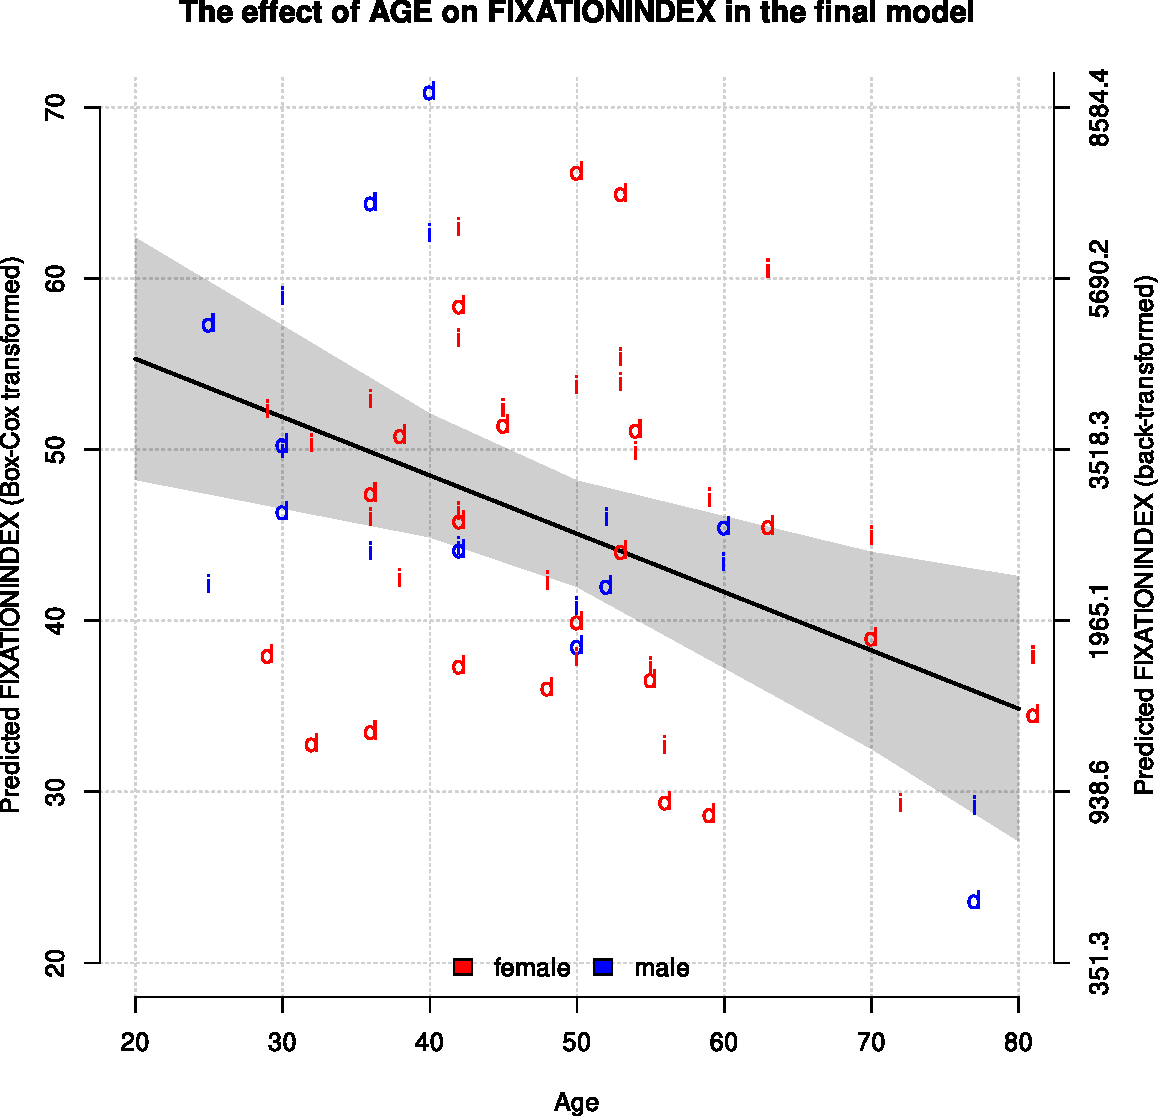
\includegraphics[height=.45\textheight]{figures/Ferreira-Figure1.1.pdf}
        \caption{Age and number of fixations\label{fig1h}}
\end{figure}

\begin{figure}
        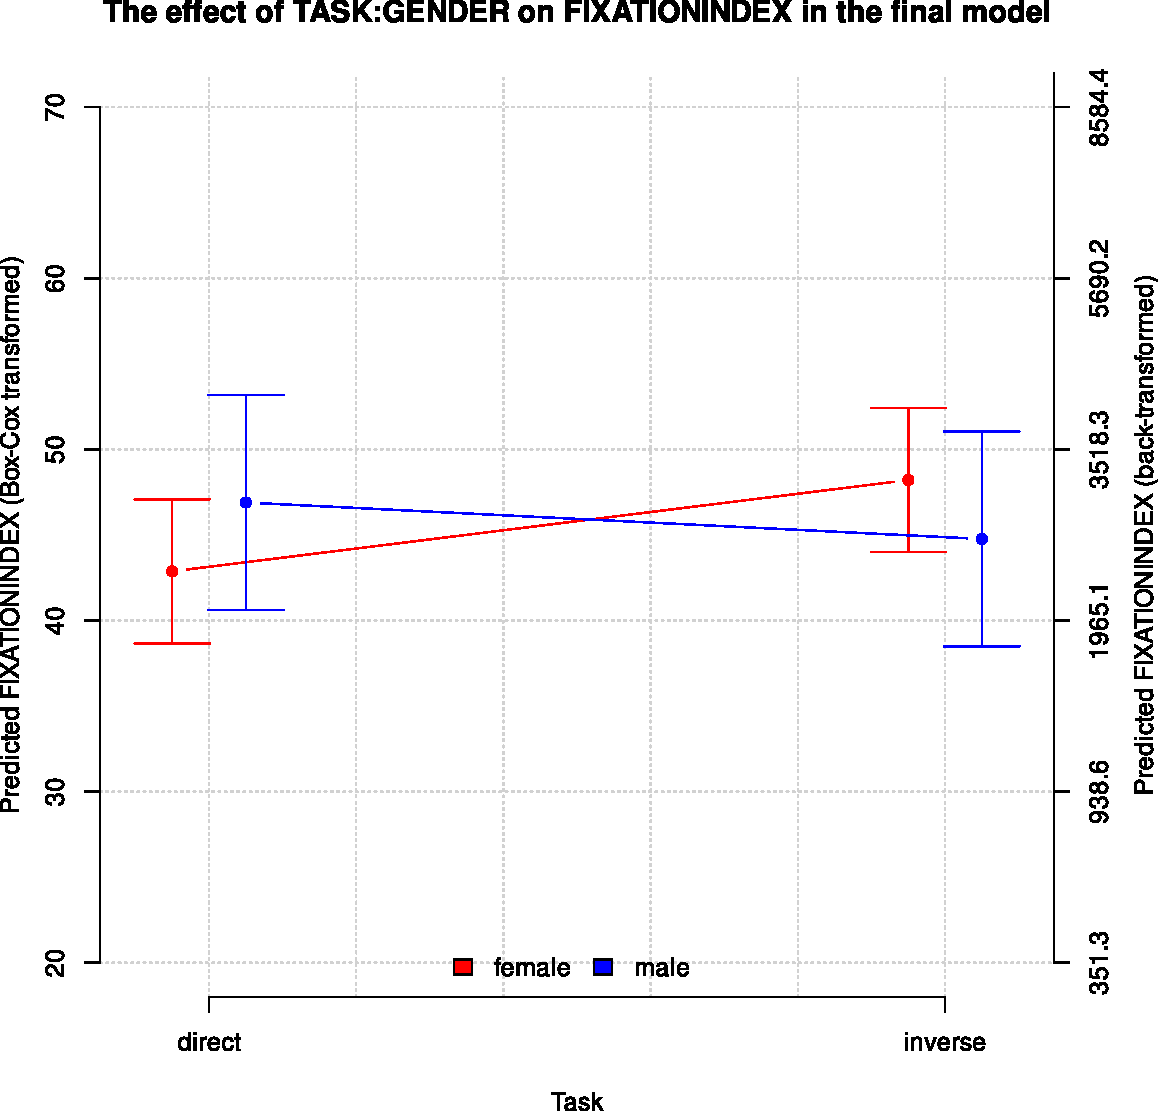
\includegraphics[height=.45\textheight]{figures/Ferreira-Figure1.2.pdf}
        \caption{Task/gender and number of fixations\label{fig2h}}
\end{figure}

For gaze event duration, the final model was significant ($\text{LR} = 16.321, \df = 1, p < 0.001$), but the correlation of TASK was only weak and most of the variability accounted for was due to individual variation ($R^2m = 0.053, R^2c = 0.078$). \figref{fig3h} shows that gaze duration was higher in IT compared to DT. 

\begin{figure}
        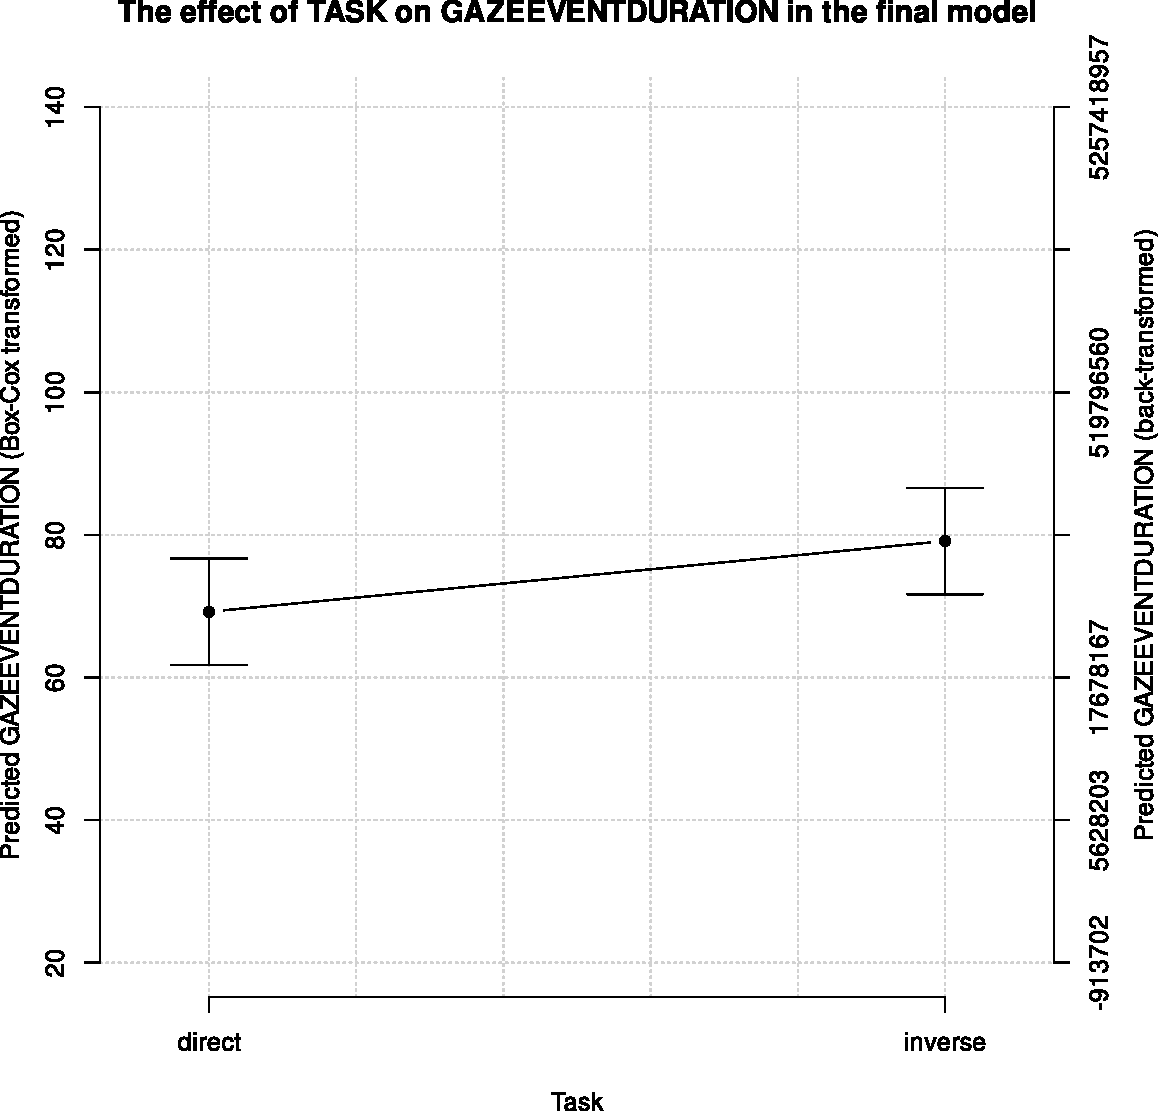
\includegraphics[height=.45\textheight]{figures/Ferreira-Figure1.3.pdf}
        \caption{Task and gaze duration\label{fig3h}}
\end{figure}

Regarding gaze point index, the final model was significant ($\text{LR} = 19.431, \df = 3, p < 0.001$) but the correlation was again not strong ($R^2m = 0.07, R^2c = 0.207$). Task and Dominance are interacting significantly such that English-dominant speakers had higher values of gaze point index during IT than DT, but Spanish-dominant speakers had higher values of gaze point index in DT compared to IT. 

In terms of keypresses, the final model was significant ($\text{LR} = 12.355, \df = 3, p < 0.001$), with a significant correlation ($R^2m = 0.112, R^2c = 0.506$) due to the interaction between Task and Dominance, English-dominant speakers had more keypresses in the IT compared to DT, but Spanish-dominant speakers had the same keypress values regardless of the direction (see \figref{fig5h}).

As per mouse events, the overall model did in fact not do significantly better than a null model, but three main effects showed significant results, leading to a decent correlation: ($R^2m = 0.281, R^2c = 0.615$). In \figref{fig6h}, a significant effect for age can be seen ($p < 0.01$): the older the subject, the lower the number of mouse events.

As shown in \figref{fig7h}, (in which the point characters d and i represent the task (direct vs. inverse) mouse events were also significantly lower for Spanish-dominant participants ($p < 0.04$). 

Mouse movements also were dependent on the task: there were more mouse movements during IT compared to DT ($p < 0.02$) (see \figref{fig8h}).

As per saccade index, the final model was significant ($\text{LR} = 23.229, \df = 4, p < 0.001$) with a decent correlation ($R^2m = 0.218, R^2c = 0.6$). The main effect for age was significant ($p < 0.01$): the older the translator, the lower is the number of saccades (\figref{fig9h}, in which the point characters d and i represent the task (direct vs. inverse)).

There was also an interaction between Task and Sex/Gender ($p < 0.05$): females had lower values of saccade index during DT than in IT. The opposite pattern was found for males, who had slightly higher values of saccade index in DT than in IT (\figref{fig10h}). 

\begin{figure}
        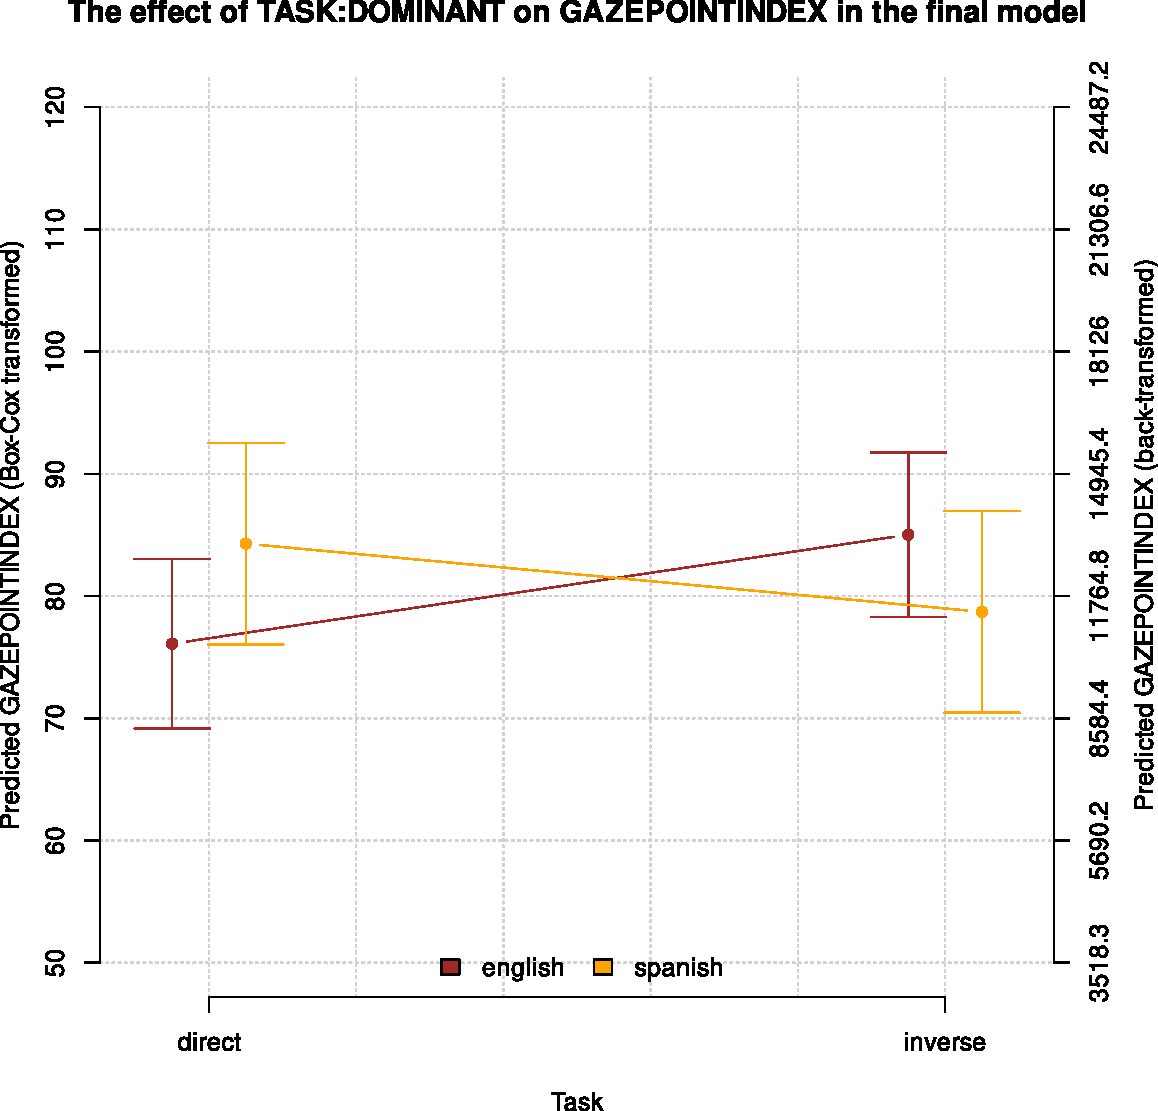
\includegraphics[height=.45\textheight]{figures/Ferreira-Figure1.4.pdf}
        \caption{Task/dominance and gaze point index\label{fig4h}}
\end{figure}

\begin{figure}
        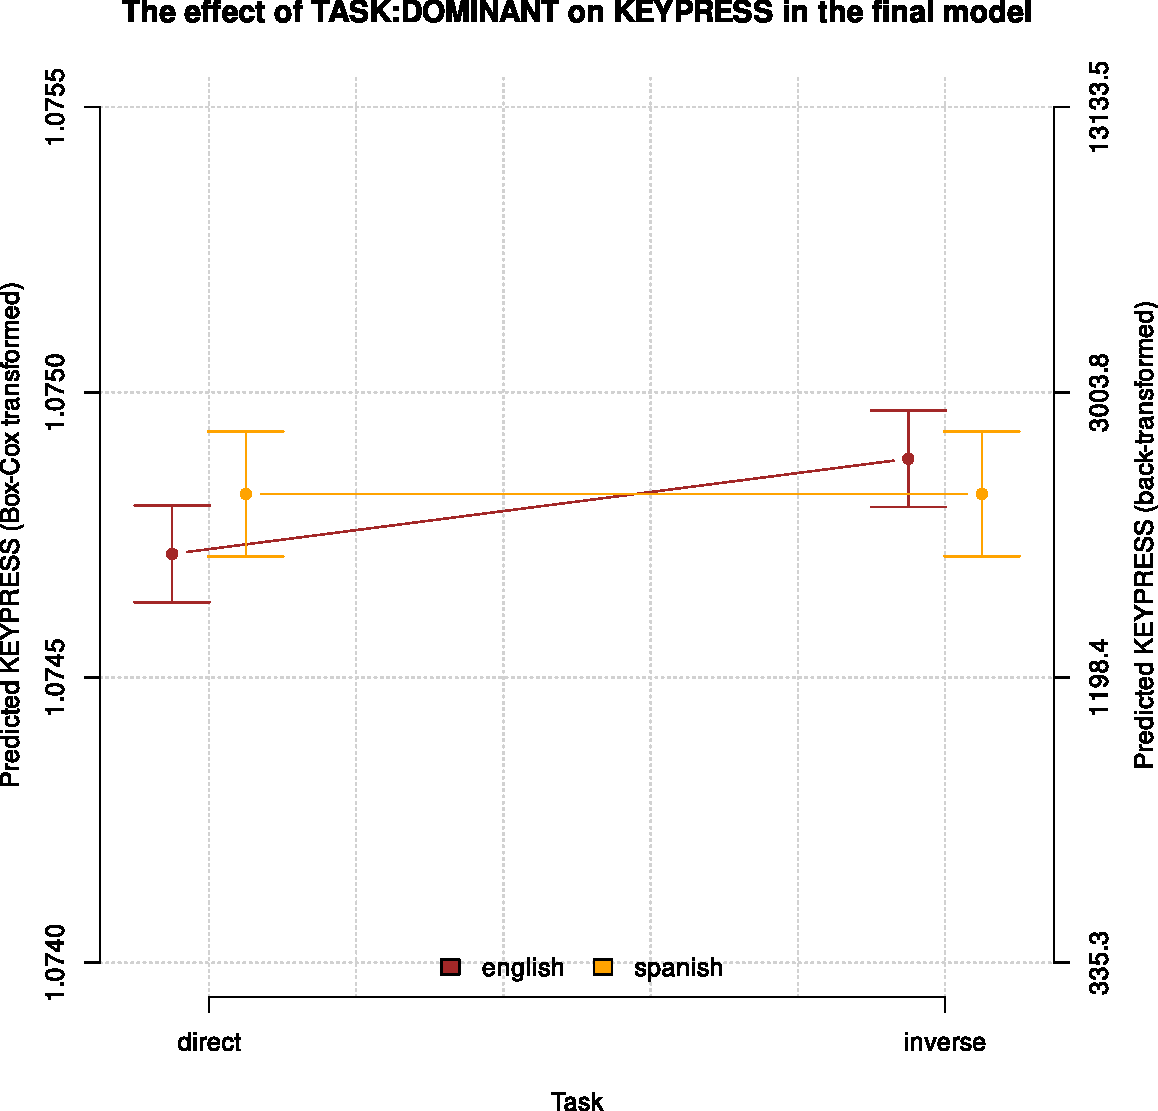
\includegraphics[height=.45\textheight]{figures/Ferreira-Figure1.5.pdf}
        \caption{Task/dominance and keypress events\label{fig5h}}
\end{figure}

\begin{figure}
        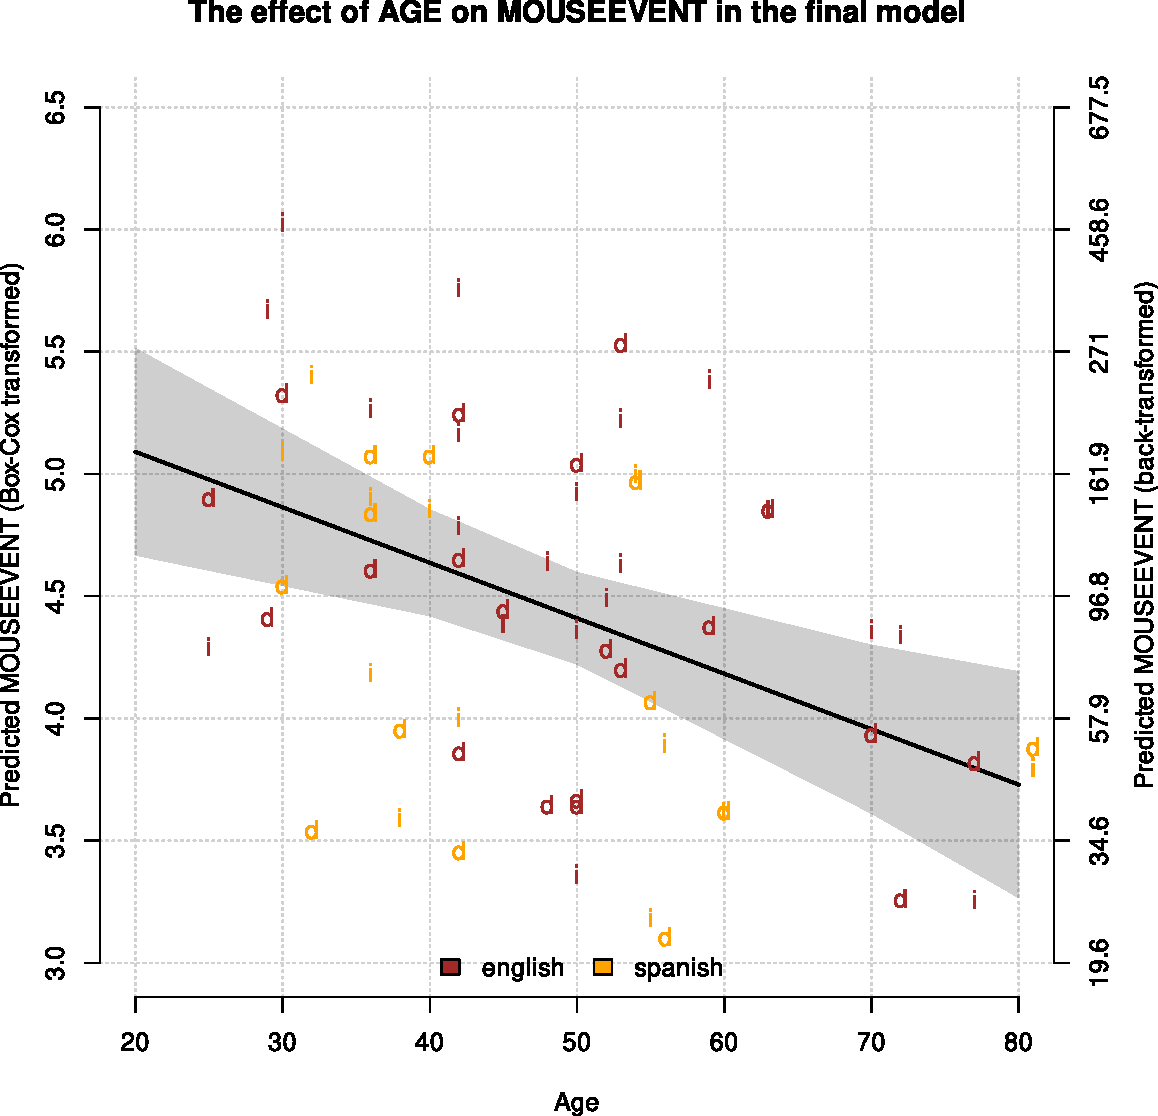
\includegraphics[height=.45\textheight]{figures/Ferreira-Figure1.6.pdf}
        \caption{Age and mouse events\label{fig6h}}
\end{figure}

\begin{figure}
        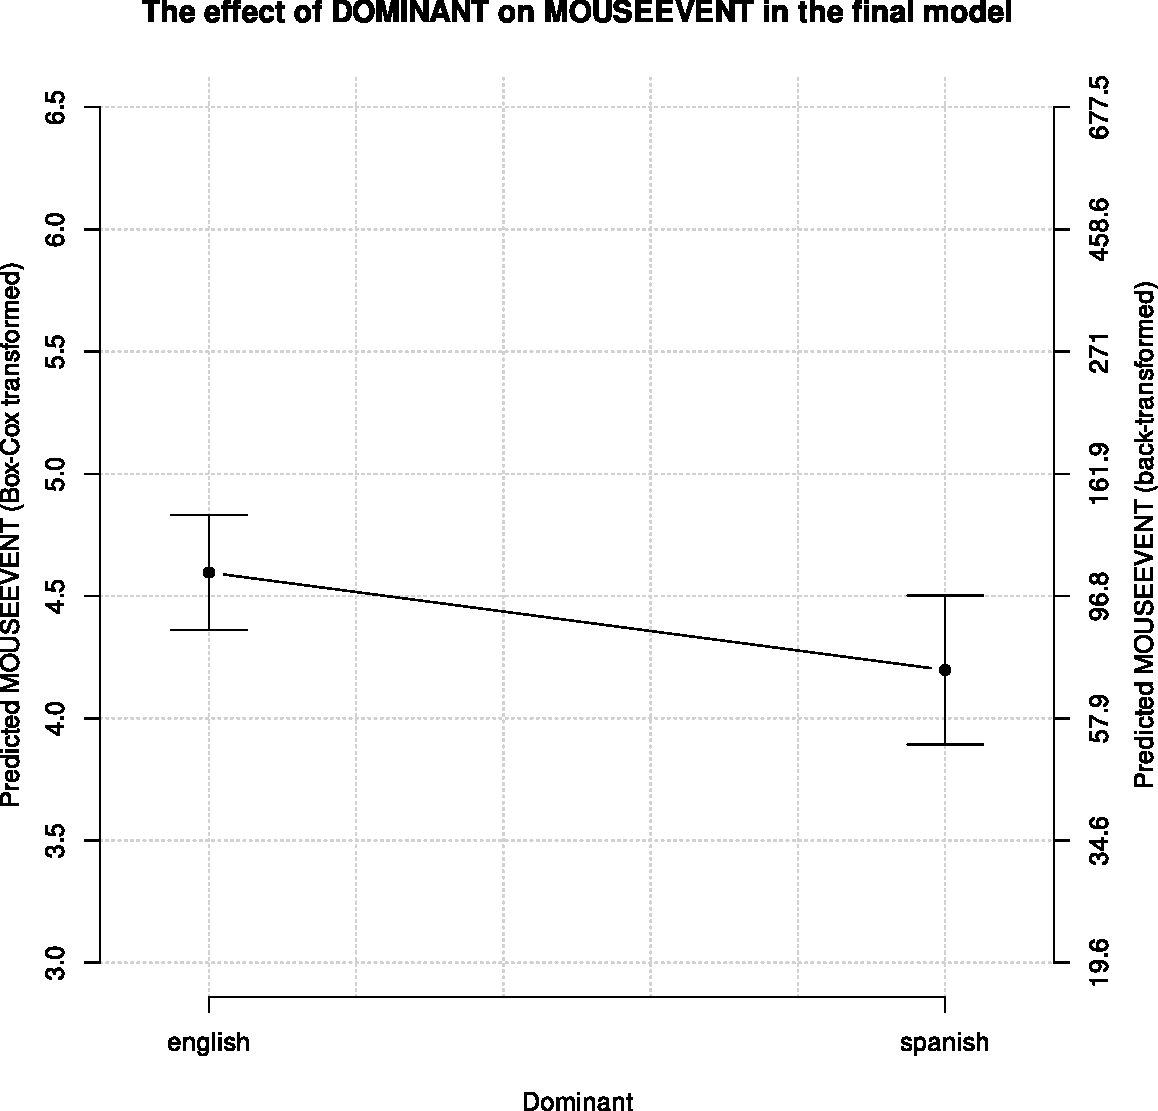
\includegraphics[height=.45\textheight]{figures/Ferreira-Figure1.7.pdf}
        \caption{Mouse events and dominance\label{fig7h}}
\end{figure}

\begin{figure}
        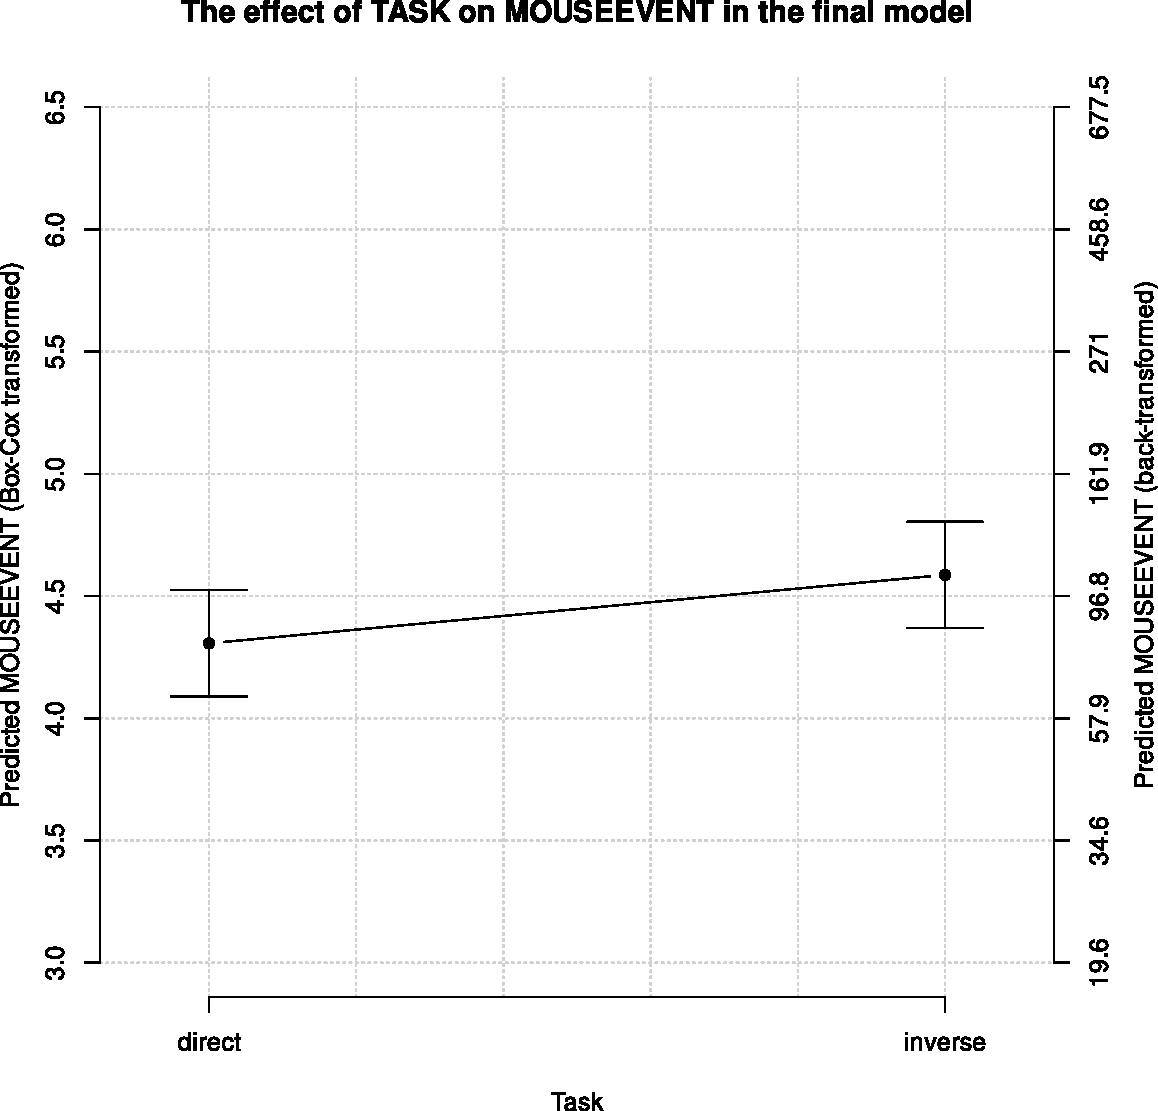
\includegraphics[height=.45\textheight]{figures/Ferreira-Figure1.8.pdf}
        \caption{Task and mouse events\label{fig8h}}
\end{figure}

\begin{figure}
        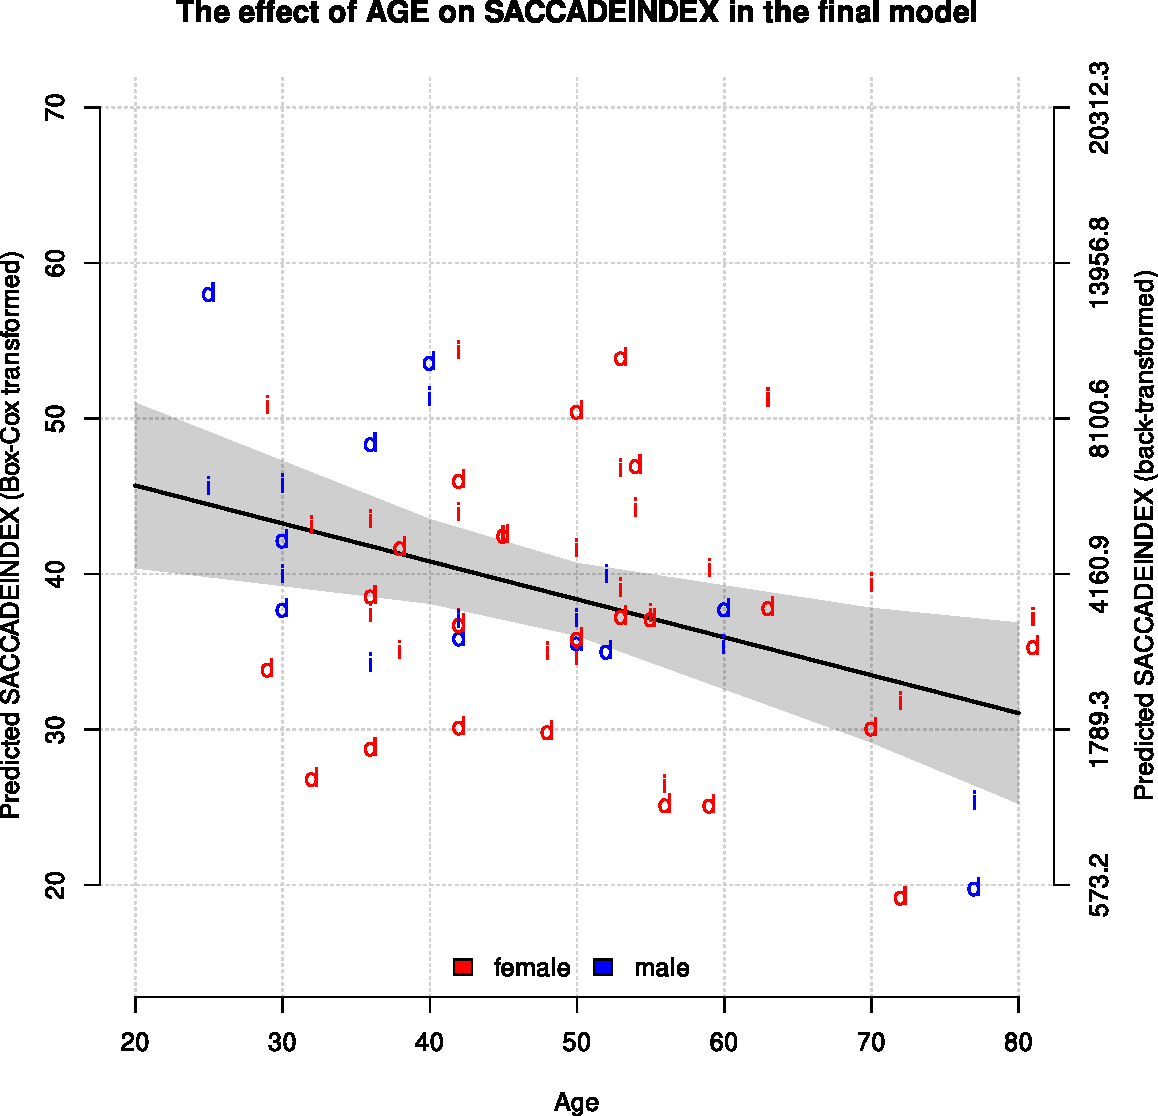
\includegraphics[height=.45\textheight]{figures/Ferreira-Figure1.9.pdf}
        \caption{Age and saccade index\label{fig9h}}
\end{figure}

\begin{figure}
        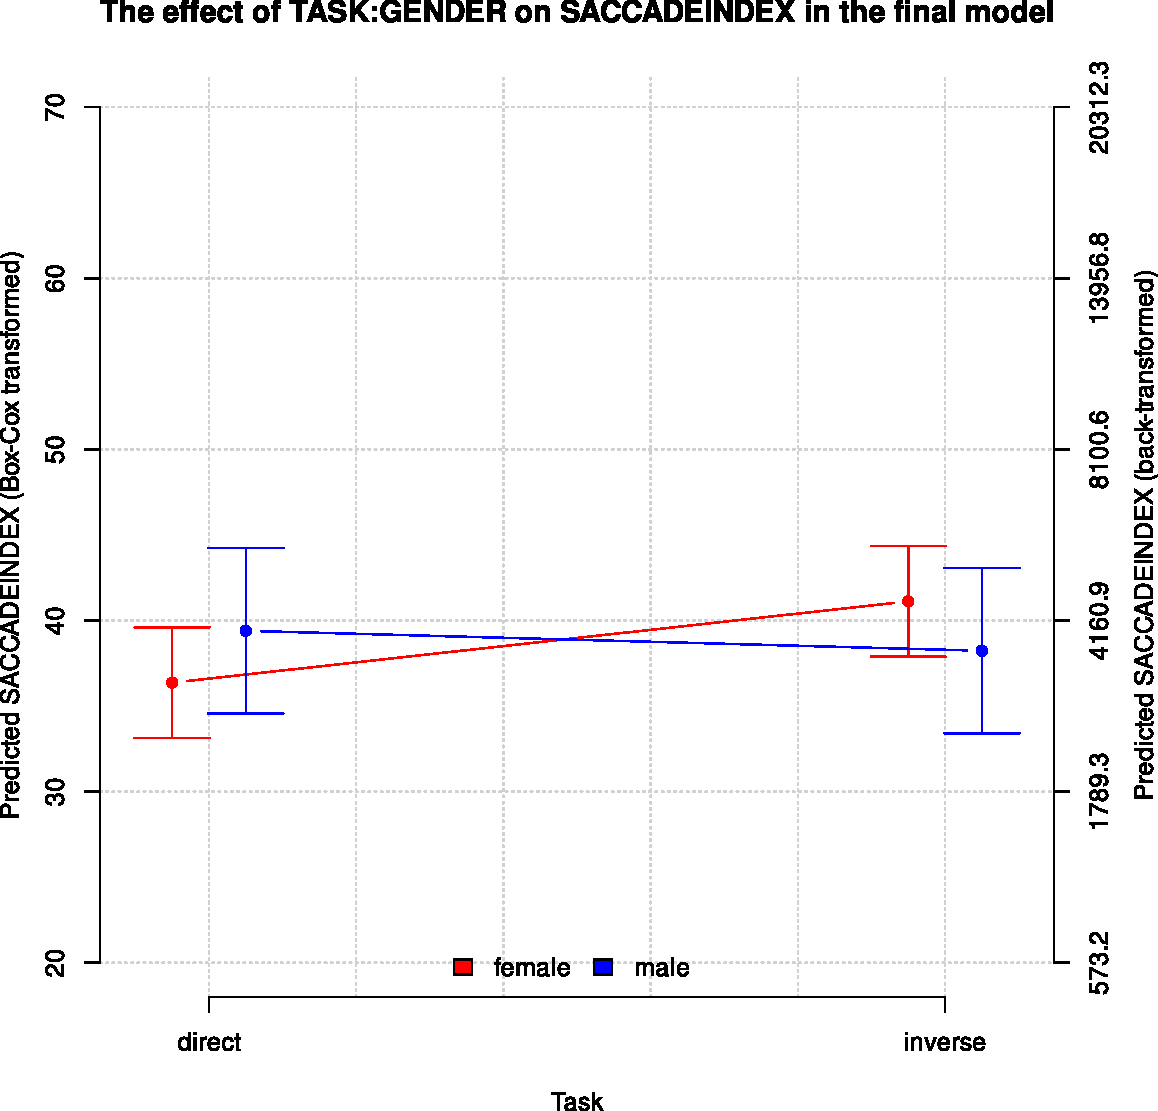
\includegraphics[height=.45\textheight]{figures/Ferreira-Figure1.10.pdf}
        \caption{Task/gender and saccade index\label{fig10h}}
\end{figure}

\clearpage
\section{Discussion}
In this study, we have provided some preliminary insight on the effects of directionality. Based on \citeauthor{ferreira2016cognitive}’s (\citeyear{ferreira2016cognitive}) analysis that took into account the total task length, fixation count, average fixation duration, and gaze time to investigate the effects of translation direction, we hypothesized that time is an indicator of cognitive effort and IT takes longer than DT. However, linear modeling for TASK (DT vs. IT) revealed no significant differences.

\citet{carl2016computational} explained that a “translator’s actions, keypresses, gaze dwell times, and mouse events, are manifestations of the translator’s cognitive states as the translation is produced.” Assuming that IT is more demanding, translators were expected to not only spend longer time in the IT but to also present higher mouse index, fixation index, gaze event duration, gaze point index, keypresses, and saccade index. With respect to fixation index, we found a correlation but the $t$-test showed no significant differences. Therefore, the variability is probably due to translators’ differences as we stated in a footnote above. Results also showed that age is correlated to fixation index (the older the subject, the lower the fixation index). This could possibly be due to a more risky reading strategy in which they are more likely than younger adults to infer the identities of upcoming works using prior context and only partial word information (\citealt{rayner2009eye}; \citealt{rayner2013eye}; \citealt{wang2018adult}).

With respect to sex/gender, our results showed that females had lower values of fixation index in IT compared to DT, whereas males presented higher values of fixation index during DT than in IT. \citet{shen2012top} investigated whether gender-based differences also existed in visual attention during a related listening task and found that men and women orient attention differently during conversational listening. Women more often exhibited “distracted saccades,” looking at the background scene element, whereas men consistently selected regions which expressed more variation in dynamic features. Further analyses will be conducted in order to analyze how those differences in DT and IT manifest in our cohort. 

As per gaze event duration, results showed that translators presented a higher gaze event duration in the IT, which suggests that gaze duration is an indicator of higher cognitive effort in the IT. On the other hand, English-dominant translators showed a higher gaze point index in IT, whereas Spanish-dominant translators presented a higher gaze point index in DT, suggesting that both groups present a higher number of gaze points when translating into Spanish. This could be due to the Spanish written system which arguably has an orthographic system that may be more demanding than that of English. Further analysis on the source text, target text, and internet browser areas of activation could shed some light to this hypothesis. 

English-dominant translators presented higher values of keypress in IT, where\-as Spanish-dominant translators showed the same amount regardless of the direction of translation. Again, it is possible that translating into Spanish may be more demanding due to its orthography. Spanish-dominant translators are more familiar with its morphosyntax and translating into Spanish might not be significantly more effortful than into English. Similarly for keypress index, Spanish-dominant translators showed a lower mouse index in both tasks, whereas mouse index is higher in the IT. Results also showed that older participants tended to use the mouse less than younger translators. \citeauthor{smith1999aging}'s (\citeyear{smith1999aging}) results showed that older participants had more difficulty performing mouse tasks in comparison to their younger peers. Differences in performance attributable to age were found in more complex tasks, and age-related changes in psychomotor abilities were related to age differences in performance. Age was also related to saccade index: the older the subject, the lower is saccade index. \citet{peltsch2011age} showed that saccadic ability decreased with age, providing insight into deficits due to normal brain changes in aging. It is likely that this is also the case in our study.

Our results also complement recent dialogues in the L2 acquisition literature. \citet{larsen2018looking} explains that “in this era of rapid change and turmoil, there are both perils and opportunities afforded by globalization” (p. 55). This suggests that researchers in the field adopt an ecological perspective to elaborate complexity guided by the relationship between variables and individual differences. Even in social approaches to language development, cognitive aspects cannot be ignored and therefore, the socio-cognitive process would provide a contribution to language development. According to Larsen-Freeman,

\begin{quote}
Socio-culturalists see social relationships as mediating learners’ cognitive development…unlike cognitive approaches, sociocognitive approaches favor patterns over rules as the object of learning, and like some of the social approaches before them, sociocognitive approaches blur the boundary between language use and its acquisition (p. 58). 
\end{quote}

\citet{larsen2018looking} further highlights the relevance of the sociopolitical context and the nature of the limitations that shape any particular acquisition context. “Language learning does not occur in an ideological vacuum but rather is affected in a serious way by prevailing beliefs held by others, including the general public” (p. 59). IT has been misconceived to be an almost impossible task~-- only being possible in cases of perfect bilingualism, without any solid empirical evidence. The fact is that people translate into the non-native language and, from what we have experienced since the first empirical studies on directionality, there is no evidence that the practice of IT will diminish moving forward simply because of beliefs or statements. 

While there are certainly “increasing complexities of language use in a global society” (\citealt[110]{kibler2016conceptualizing}), we should also reflect on how translation situates itself in society. In translation studies, for instance, language differences should be taken into account when designing studies and interpreting results. Defining one’s L1 and L2 is not an easy task: home country language, family language, and primary language of use, all of which is a common practice in fields such as developmental psychology and L2 acquisition, might have an impact on how we perceive translator’s performance. In a similar way, we should also attempt to analyze less examined variables that could possibly account for variances among participants.

\section{Conclusion}
Although previous studies \citep{ferreira2016cognitive,ferreira2018decision} suggested that language direction might have an impact on time spent in DT and IT tasks, the present study demonstrates that individual differences between subjects (including ones related to language experience), but also across subject groups such as dominance, modulate these effects. These individual differences are crucial to examine when analyzing translators’ performance and drawing conclusions, and these effects require multifactorial mixed-effects modeling of a kind that is not yet widespread in translation studies. Our sample is formed by a heterogeneous group in which professional translators’ age and experience vary, which might impact our analyses. However, eye-tracking data showed that variables other than time can be used to measure effort in translation. Not only can studying directionality help us to better understand patterns in translation, but language typology might also illuminate things. Furthermore, age and sex/gender -- used here as controlled variables -- should also be further analyzed to test whether any difference can be due to the factors. As this is an ongoing project, more data will be collected to create more homogeneous subgroups.

{\sloppy\printbibliography[heading=subbibliography,notkeyword=this]}
\end{document}
